\chapter{System Model and Architecture}
%%%%%%%%%%%%%%%%%%%%%%%%%%%%%%%%%%%%%%%%%
\section{Introduction}
This chapter presents the system model, architectural design, and module decomposition of \projname{}. It covers the frozen operational workflow, the layered architecture, individual layer responsibilities, and the module-level decomposition of the system.

%%%%%%%%%%%%%%%%%%%%%%%%%%%%%%%%%%%%%%%%%
\section{Frozen Operational Workflow}
%%%%%%%%%%%%%%%%%%%%%%%%%%%%%%%%%%%%%%%%%
The system uses a fixed Import $\rightarrow$ Encrypt $\rightarrow$ Lock $\rightarrow$ Export workflow. Files are imported into the vault as copies, not moved. They are then encrypted inside the container. The vault is locked when not in use. If the user needs a file outside the vault, it must be exported. Exported files are not protected by the vault after export.

\begin{figure}[h]
	\centering
	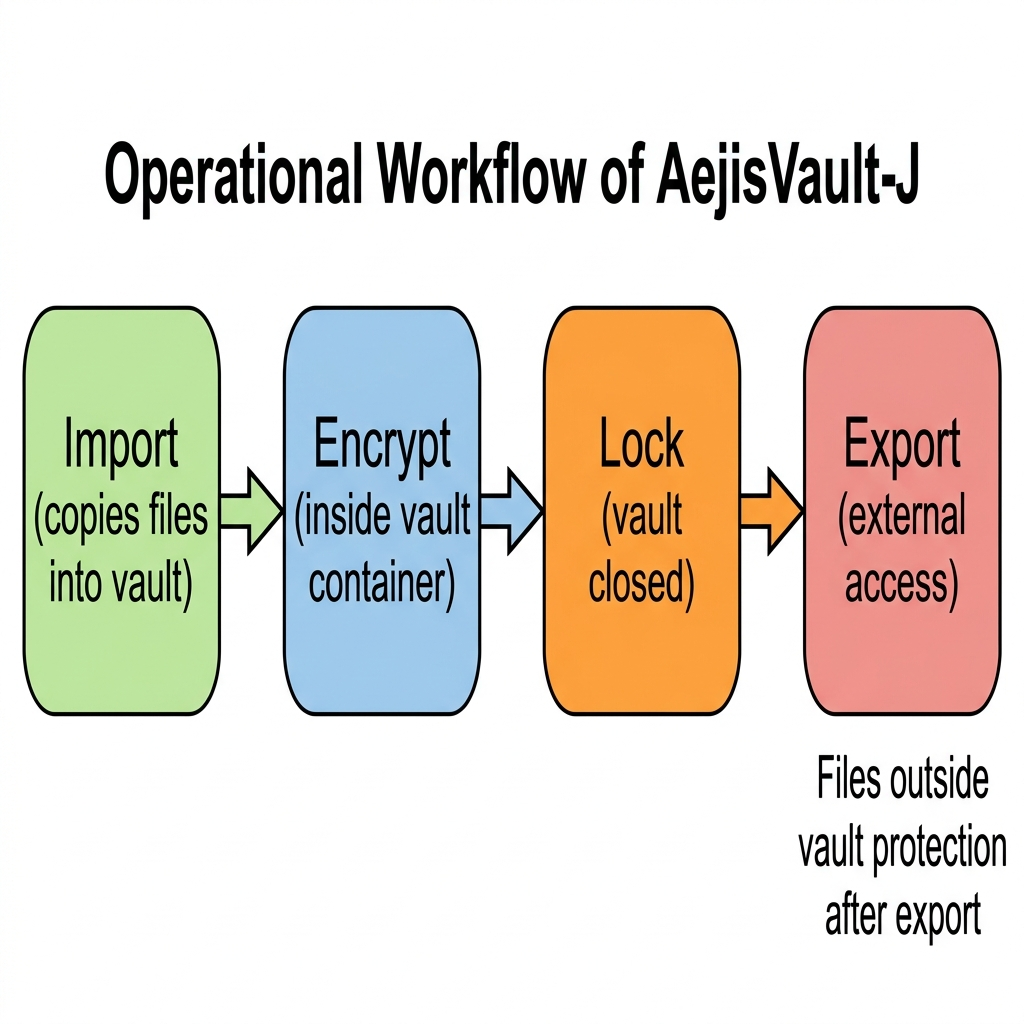
\includegraphics [width=0.85\textwidth] {figures/operational_workflow}
	\caption{Operational workflow of \projname{}. The vault enforces a deliberate sequence of actions rather than hidden background encryption.}
	\label{fig:workflow}	
\end{figure}

%%%%%%%%%%%%%%%%%%%%%%%%%%%%%%%%%%%%%%%%%
\section{Security Consequences of the Model}
%%%%%%%%%%%%%%%%%%%%%%%%%%%%%%%%%%%%%%%%%
This workflow creates a clear line between protected and unprotected data. It helps users understand that the vault protects files only while they remain inside it. It also prevents a common misconception that an encryption tool automatically secures copies placed elsewhere on the host system. The exported file is ordinary file data and must be protected separately if needed.

%%%%%%%%%%%%%%%%%%%%%%%%%%%%%%%%%%%%%%%%%
\section{What the System Is}
%%%%%%%%%%%%%%%%%%%%%%%%%%%%%%%%%%%%%%%%%
\projname{} is a digital safe for files, a portable encrypted container with the .avj extension, a Java-based cross-platform application, and a logically structured virtual file system.

%%%%%%%%%%%%%%%%%%%%%%%%%%%%%%%%%%%%%%%%%
\section{What the System Is Not}
%%%%%%%%%%%%%%%%%%%%%%%%%%%%%%%%%%%%%%%%%
The system is not disk encryption, not a mounted filesystem, not real-time file encryption, not protection for exported files, and not malware-resistant in the sense that a compromised host remains compromised. These exclusions are important because they prevent misleading security assumptions.

%%%%%%%%%%%%%%%%%%%%%%%%%%%%%%%%%%%%%%%%%
\section{Layered Architecture}
%%%%%%%%%%%%%%%%%%%%%%%%%%%%%%%%%%%%%%%%%
The architecture of the system is organized into five layers: JavaFX UI layer, service layer, virtual file system layer, encryption engine layer, and container file layer. Each layer has a narrow responsibility and communicates with adjacent layers through explicit interfaces. The layered architecture is shown in Figure \ref{fig:architecture}.

\begin{figure}[h]
	\centering
	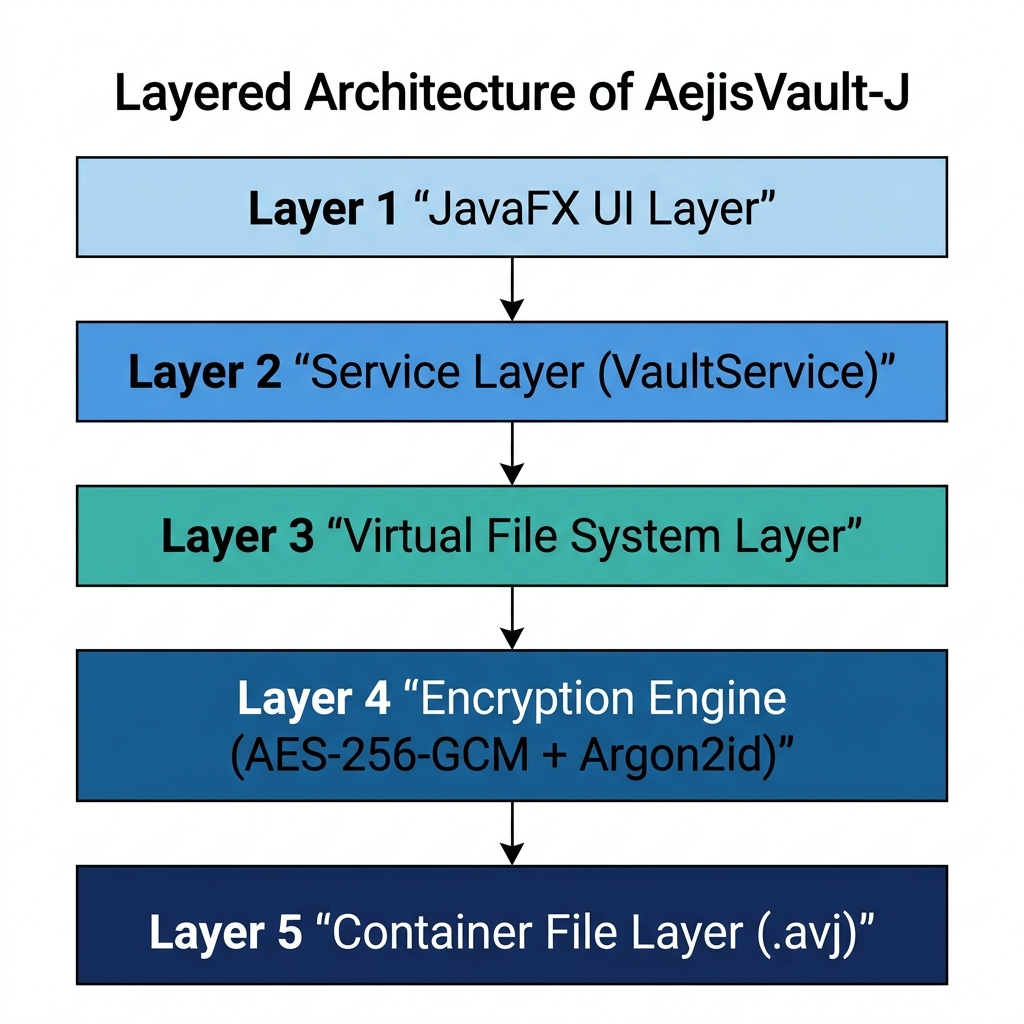
\includegraphics [width=0.85\textwidth] {figures/system_architecture}
	\caption{Layered architecture of \projname{}. The design separates presentation, business logic, logical file organization, cryptography, and persistent storage.}
	\label{fig:architecture}	
\end{figure}

%%%%%%%%%%%%%%%%%%%%%%%%%%%%%%%%%%%%%%%%%
\section{JavaFX UI Layer}
%%%%%%%%%%%%%%%%%%%%%%%%%%%%%%%%%%%%%%%%%
The user interface is implemented with JavaFX \index{JavaFX}. Its role is to present vault actions, accept credentials, show folder hierarchy, display security warnings, and guide the user through import and export flows. The UI layer must not perform cryptographic operations directly; instead, it delegates to the service layer.

%%%%%%%%%%%%%%%%%%%%%%%%%%%%%%%%%%%%%%%%%
\section{Service Layer}
%%%%%%%%%%%%%%%%%%%%%%%%%%%%%%%%%%%%%%%%%
The \texttt{VaultService} coordinates application behavior. It validates user actions, enforces state transitions, and invokes file and cryptography operations in the proper order. Keeping these tasks in a service layer helps reduce coupling between UI elements and security-sensitive operations.

%%%%%%%%%%%%%%%%%%%%%%%%%%%%%%%%%%%%%%%%%
\section{Virtual File System Layer}
%%%%%%%%%%%%%%%%%%%%%%%%%%%%%%%%%%%%%%%%%
The virtual file system \index{Virtual file system} models the internal structure of the vault. It is logical rather than mounted at the operating system level. This design choice avoids kernel integration and reduces implementation complexity while still supporting folders and nested content.

%%%%%%%%%%%%%%%%%%%%%%%%%%%%%%%%%%%%%%%%%
\section{Encryption Engine Layer}
%%%%%%%%%%%%%%%%%%%%%%%%%%%%%%%%%%%%%%%%%
The encryption engine handles authenticated encryption, key generation, key derivation, key wrapping, and secure deletion attempts. It is the most security-sensitive layer and therefore requires careful testing and review.

%%%%%%%%%%%%%%%%%%%%%%%%%%%%%%%%%%%%%%%%%
\section{Container File Layer}
%%%%%%%%%%%%%%%%%%%%%%%%%%%%%%%%%%%%%%%%%
The .avj file is the persistent vault container. It stores encrypted metadata, encrypted content blobs, and cryptographic parameters required for opening the vault. Since the container is a single file, it is portable and can be transferred or backed up easily.

%%%%%%%%%%%%%%%%%%%%%%%%%%%%%%%%%%%%%%%%%
\section{Module Design}
%%%%%%%%%%%%%%%%%%%%%%%%%%%%%%%%%%%%%%%%%
The system is decomposed into four modules, each with a distinct responsibility. The module design is shown in Figure \ref{fig:module_design}.

\begin{figure}[h]
	\centering
	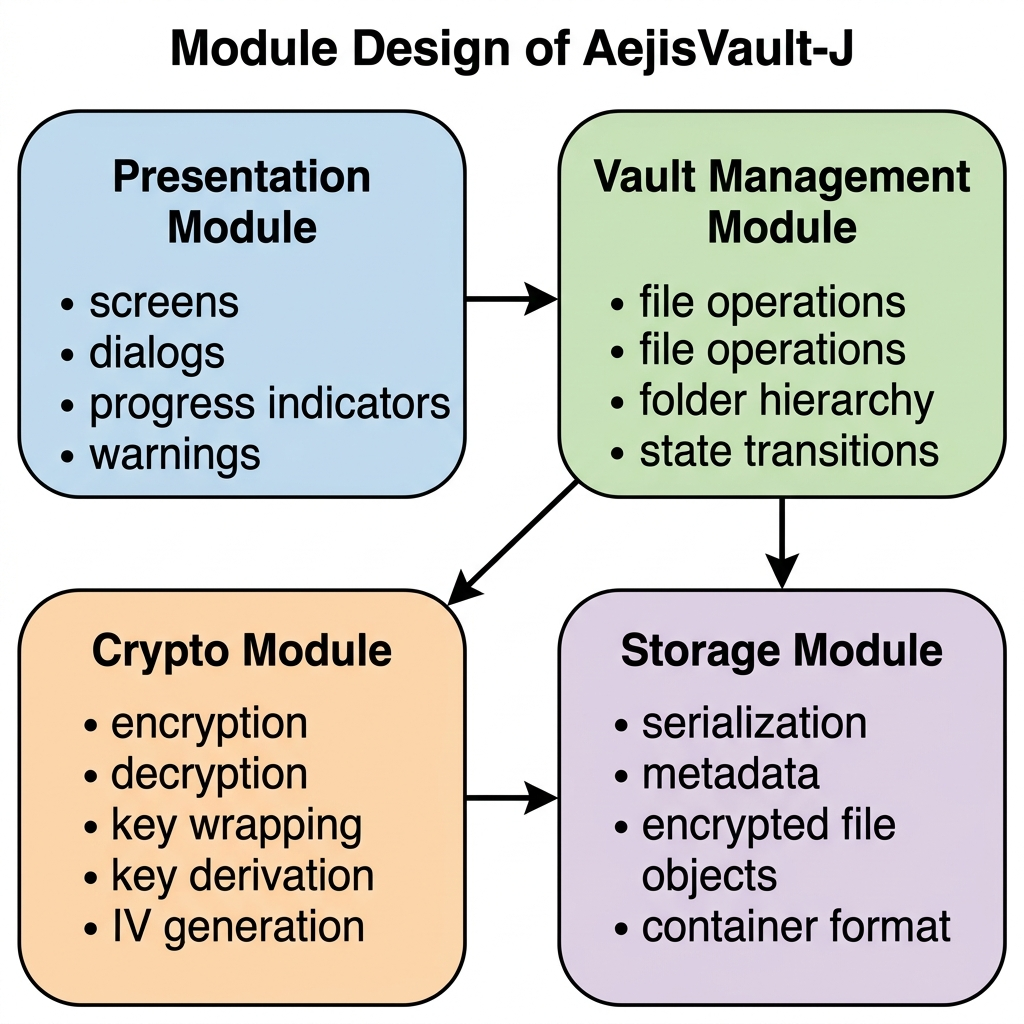
\includegraphics [width=0.85\textwidth] {figures/module_design}
	\caption{Module design of \projname{} showing the four core modules and their interactions.}
	\label{fig:module_design}	
\end{figure}

\subsection{Presentation Module}
The presentation module is responsible for screens, dialog boxes, progress indicators, warning messages, and user interaction events. It must remain free from direct cryptographic implementation details.

\subsection{Vault Management Module}
The vault management module coordinates file operations, folder hierarchy updates, and state transitions between open, locked, and exported states.

\subsection{Crypto Module}
The crypto module performs encryption, decryption, key wrapping, key derivation, and initialization vector generation. It must be isolated and well tested because errors here directly affect security.

\subsection{Storage Module}
The storage module serializes metadata, encrypted file objects, and integrity-protected headers into the container file format. It also reconstructs them when opening the vault.

%%%%%%%%%%%%%%%%%%%%%%%%%%%%%%%%%%%%%%%%%
\section{Enhanced Modules (Major Project)}
%%%%%%%%%%%%%%%%%%%%%%%%%%%%%%%%%%%%%%%%%
In the major project phase, four additional modules were integrated into the existing architecture, each adding significant enterprise-grade capability while preserving the original layered design.

\subsection{Audit Module}
The audit module (\texttt{com.aegisvault.audit}) records every security-relevant operation performed within the vault. It tracks events such as vault creation, vault opening and closing, file imports, file deletions, file renames, password changes, and key protection mode changes. Each audit event is timestamped and stored within the encrypted vault itself, ensuring that the audit trail is protected by the same cryptographic guarantees as the vault data. A dedicated \texttt{AuditLogViewer} UI provides searchable, filterable, and exportable access to the audit trail.

\subsection{Hardware Key Protection Module}
The hardware key protection module (\texttt{com.aegisvault.crypto}) enables the use of OS-level keystores for wrapping and unwrapping the Master Vault Key. On Windows, this leverages the \texttt{Windows-ROOT} keystore; on macOS, the \texttt{KeychainStore}; and on Linux, PKCS\#11 when available. The module supports three modes: software-only (default), OS keystore, and OS keystore with software fallback. This provides defense-in-depth by binding vault keys to the platform's trusted hardware or secure enclave.

\subsection{Cloud Synchronization Module}
The cloud synchronization module (\texttt{com.aegisvault.sync}) enables encrypted vault files to be synchronized to remote storage. Two providers are implemented: local folder synchronization (for network shares and external drives) and WebDAV synchronization (for cloud-based storage). The \texttt{SyncEngine} handles upload, download, and conflict detection. Synchronization can be triggered manually, on vault close, or on a scheduled interval. Enterprise policies can disable synchronization entirely.

\subsection{Enterprise Deployment Module}
The enterprise deployment module (\texttt{com.aegisvault.enterprise}) supports organizational deployment of \projname{}. It includes a cascading configuration loader that reads policies from application defaults, user home directory, system-wide configuration, and Windows registry (Group Policy). Enterprise administrators can enforce minimum password lengths, maximum auto-lock timeouts, allowed ciphers, and synchronization permissions. The module also includes multi-vault management with health checks, silent installation configuration, and deployment report generation for IT administrators.
